\newpage
\section{Comparador con Histéresis}
\onehalfspacing
\begin{figure}[htb]
	\centering
	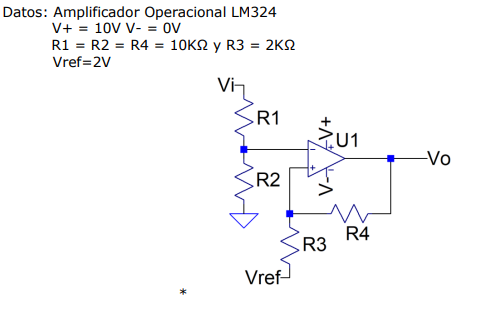
\includegraphics[width=1\textwidth]{figuras/Circuito4_consigna.png}
	\caption{Circuito propuesto}
\end{figure}
En este circuito está el AO LM324 operando con realimentación positiva en configuracion "Schmitt trigger inversor", implementado con fuente alimentación asimétrica 0 a 10 [V].
\subsection{Análisis teórico}
Para un análisis mas detallado se considera el caso general con alimentación simétrica y que el A.O. no sea del tipo Rail to Rail. Se analiza $V_o$ a partir de la tensión diferencial $V_d$ y por último se analiza el caso particular con $V_{ss}=0$.\\
Se definen $v^+$ y $v^-$ de la siguiente manera:
\begin{center}
	$v^- = k_1 * V_{in}$
\end{center}
\begin{center}
	$v^+ = k_2 * (V_o - V_{ref})+V_{ref}$
\end{center}
teniendo que:
\begin{center}
	$k_1 = \frac{R_2}{R_1 + R_2}$
\end{center}
\begin{center}
	$k_2 = \frac{R_3}{R_3 + R_4}$
\end{center}

\subsubsection{Si $V_d<0$}
Para un A.O ideal si $V_d<0$ la salida del amplificador debería ser $V_{ss}$
\begin{center}
	
	$V_d = (v^+ - v^-)<0 \rightarrow  V_o = V_{ss}$
\end{center}
entonces
\begin{center}
	$v^+ < v^-$
\end{center}
\begin{center}
	$k_2 * (v_o - v_{ref})+ v_{ref} < k_1 * v_{in}$
\end{center}
\begin{center}
	$\frac{k_2}{k_1} * (v_o- v_{ref}) + \frac{v_{ref}}{k_1} <v_{in}$ 
\end{center}
\begin{center}
	$\frac{k_2}{k_1} * v_o + \frac{1 - k_2}{k_1} * v_{ref} <v_{in}$ 
\end{center}

\begin{center}
	$\left\{\begin{matrix}
	v_o = v_{cc}\\ 
	v_{cc} = 10[V]\\ 
	v_{ref} = 2[V]\\ 
	R_3 = 2[K\Omega]\\ 
	R_1 = R_2 = R_3 = 10[K\Omega]
\end{matrix}\right.$
\end{center}
\begin{center}
	$v_{in} > 6.67[V] \rightarrow v_o = v_{ss}$ 
\end{center}

\subsubsection{Si $V_d>0$}
Para un A.O ideal si $V_d>0$ la salida del amplificador debería ser $V_{cc}$
\begin{center}
	
	$V_d = (v^+ - v^-)>0 \rightarrow  V_o = V_{cc}$
\end{center}
entonces
\begin{center}
	$v^+ > v^-$
\end{center}
\begin{center}
	$k_2 * (v_o - v_{ref})+ v_{ref} > k_1 * v_{in}$
\end{center}
\begin{center}
	$\frac{k_2}{k_1} * (v_o- v_{ref}) + \frac{v_{ref}}{k_1} > v_{in}$ 
\end{center}
\begin{center}
	$\frac{k_2}{k_1} * v_o + \frac{1 - k_2}{k_1} * v_{ref} > v_{in}$ 
\end{center}

\begin{center}
	$\left\{\begin{matrix}
		v_o = v_{ss}\\ 
		v_{ss} = -10[V]\\ 
		v_{ref} = 2[V]\\ 
		R_3 = 2[K\Omega]\\ 
		R_1 = R_2 = R_3 = 10[K\Omega]
	\end{matrix}\right.$
\end{center}
\begin{center}
	$v_{in} < 0[V] \rightarrow v_o = v_{cc}$ 
\end{center}
resumiendo entonces lo obtenido:
\begin{center}
	$v_o(v_{in}) = \left\{\begin{matrix}
		v_{cc}$ para $v_{in} < 0[V]\\ 
		v_{ss}$ para $v_{in} > 6.67[V]
	\end{matrix}\right.$
\end{center}
\subsubsection{Si $V_{ss} = 0$}
Para este caso particular la relación queda 
\begin{center}
	$\frac{1 - k_2}{k_1} * v_{ref} > v_{in}$
\end{center}
donde se ve que el punto de conmutación queda directamente dependiente de $v_{ref}$.
\begin{center}
	Reemplazando $\left\{\begin{matrix}
		v_{ref} = 2[V] \\
		R_3 = 2[K\Omega] \\
		R_1 = R_2 = R_4 10[K\Omega]
	\end{matrix}\right.$
\end{center}
\begin{center}
 Si: $v_{in} < 3.33[V] \rightarrow v_o = v_{ss}$
\end{center}
Los análisis anteriores son válidos para un amplificador ideal o de tipo Rail to Rail, en este caso obtenido por simulación la salida máxima del LM324 es de 8.5[V], entonces queda:
\begin{center}
	Si: $v_{in} > 6.17[V] \rightarrow v_o = v_{cc}$
\end{center}
Finalmente para el LM324 y $v_{ss}=0$
\begin{center}
	$v_o(v_{in}) = \left\{\begin{matrix}
		v_{cc}$ para $v_{in} < 3.33[V]\\ 
		v_{ss}$ para $v_{in} > 6.77[V]
	\end{matrix}\right.$
\end{center}


\subsection{Simulación}
\begin{figure}[H]
	\centering
	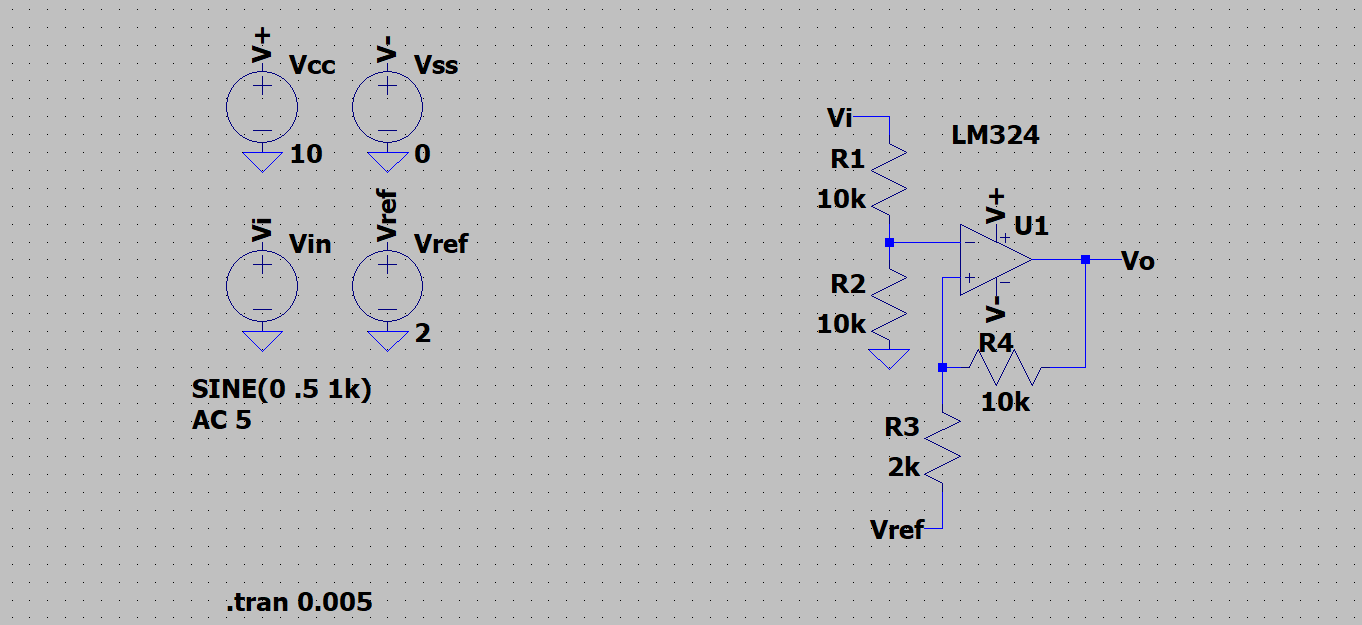
\includegraphics[width=1\textwidth]{figuras/Circuito4.png}
	\caption{Circuito simulado}
\end{figure}
\subsubsection{Caso general $v_{cc}$ y $v_{ss}$ distintos de cero y simétricos}
\begin{figure}[H]
	\centering
	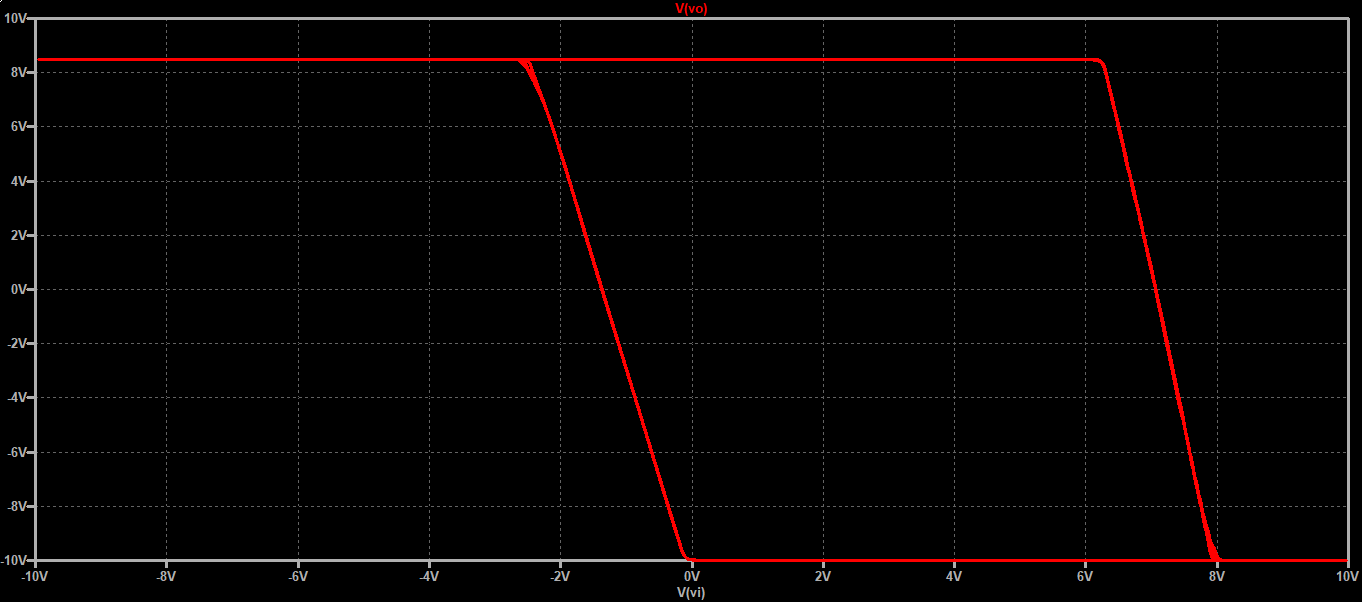
\includegraphics[width=1\textwidth]{figuras/caso_gral_histeresis.png}
	\caption{$Vo_1= f(v_{in})$ con $V_{in}$ = 10 [V] y 1[KHz].}
\end{figure}
\begin{figure}[H]
	\centering
	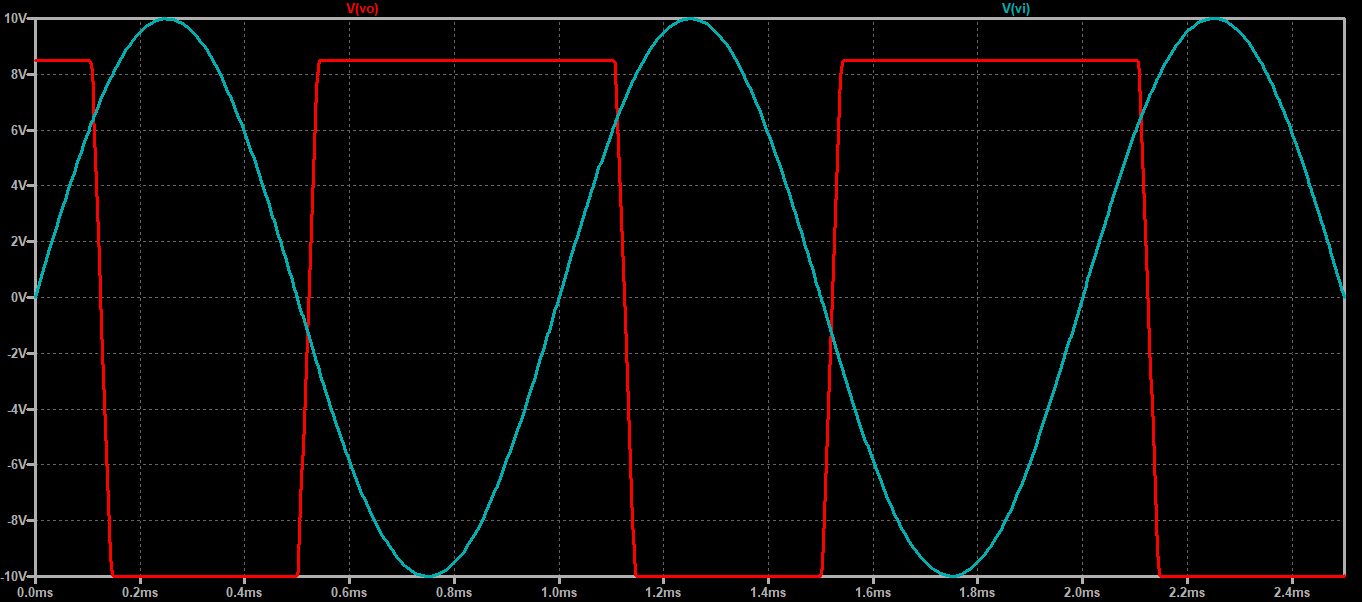
\includegraphics[width=1\textwidth]{figuras/caso_gral_histeresis_time.png}
	\caption{$Vo_1= f(v_{in})$ con $V_{in}$ = 10 [V] y 1[KHz] en el tiempo.}
\end{figure}

\subsubsection{Caso general $v_{cc}$10[V] y $v_{ss}$0[V] distintos de cero y simétricos}
\begin{figure}[H]
	\centering
	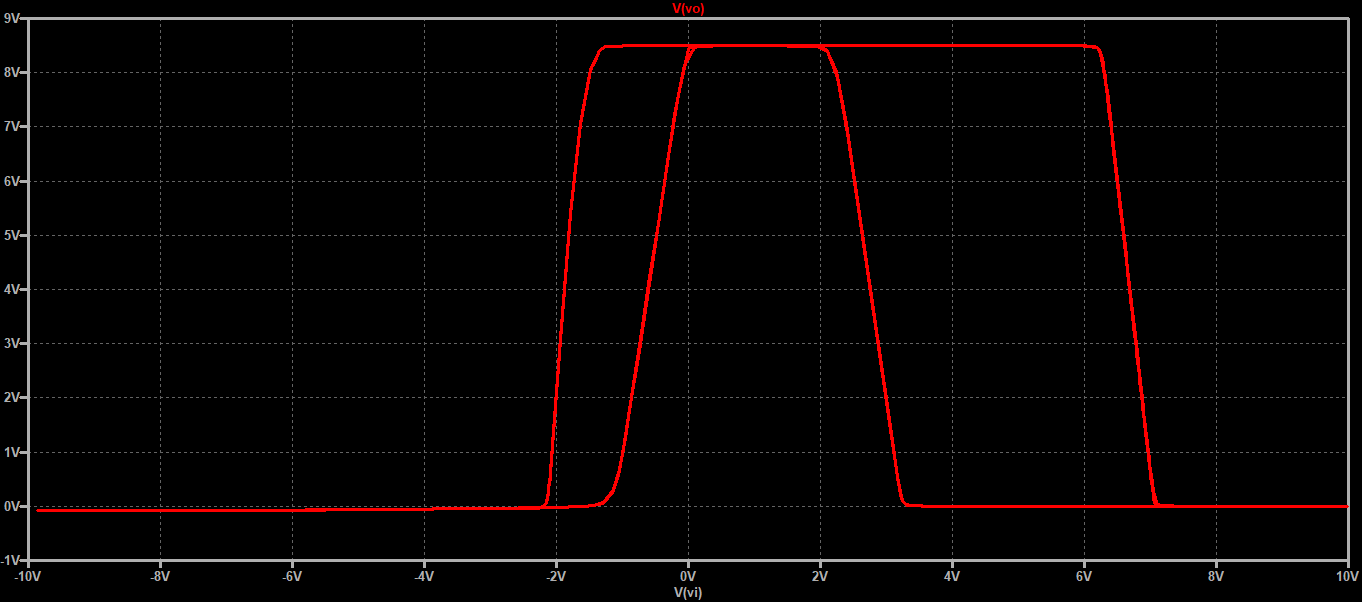
\includegraphics[width=1\textwidth]{figuras/caso_vss=0_histeresis.png}
	\caption{$Vo_1= f(v_{in})$ con $V_{in}$ = 10 [V] y 1[KHz].}
\end{figure}
\begin{figure}[H]
	\centering
	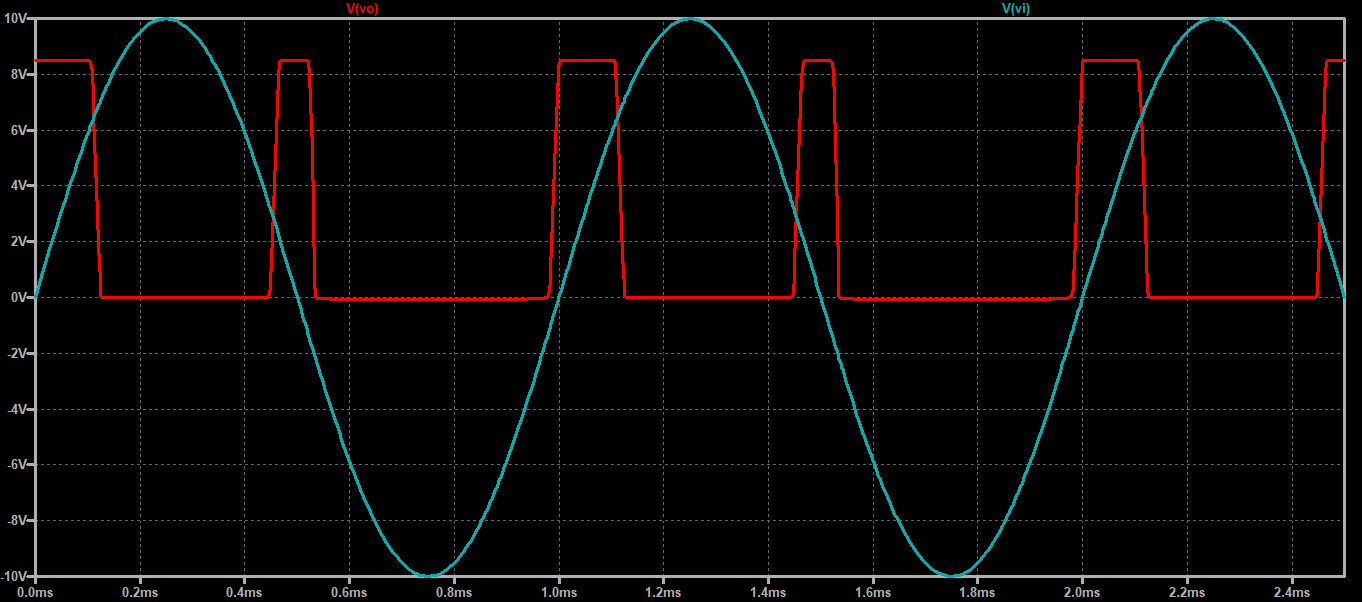
\includegraphics[width=1\textwidth]{figuras/caso_vss=0_histeresis_time.png}
	\caption{$Vo_1= f(v_{in})$ con $V_{in}$ = 10 [V] y 1[KHz] en el tiempo.}
\end{figure}